\documentclass[12pt,a4paper]{article}
\usepackage{../style}


\newcommand{\titDoc}{Piano di Qualifica}
\newcommand{\dataCreazione}{05 Gennaio 2015}
\newcommand{\versione}{2.0}
\newcommand{\stato}{Formale}
\newcommand{\uso}{Esterno}

\lfoot{
	\titDoc \\
	v. \versione
}
\title{\titDoc}

\begin{document}
\thispagestyle{empty}

\begin{titlepage}
	\begin{center}
	\begin{Huge}
		\textbf{\gruppo} \\
	\end{Huge}
	\vspace{0.5cm}
	\begin{Large}
		\textbf{\capitolato}
	\end{Large}
	
	\vspace{1cm}
    
	
\includegraphics[scale=0.35]{../logo/logo404_Extends.png}
	\vspace{1cm}
	\begin{Huge}
		\textbf{\titDoc}
	\end{Huge}
	
	\vspace{1cm}
	\textbf{Informazioni sul documento}\\
    \rule{10cm}{.4pt} \\
	\begin{table}[h]
	\begin{center}
	\begin{tabular}{r | l}
<<<<<<< HEAD
		\textbf{Versione} & \versione \\ \\
=======
		\textbf{Versione} & 2.0 \\ \\
>>>>>>> origin/master
		\textbf{Redazione} & \CoMa \\
			& \ReAn \\ 
			& \DeEn \\ 
			& \CaMa \\ \\
		\textbf{Verifica} &\MaMo \\ \\
		\textbf{Responsabile} & \GoIs \\ \\
		\textbf{Uso} & Interno \\ \\
		\textbf{Ultima modifica} & 25 Marzo 2015 \\ \\
		\textbf{Lista di distribuzione} & \gruppo \\ 
	\end{tabular}
	\end{center}
	\end{table}
			\textbf{Descrizione} \\
			Documento contenente le norme stabilite dal gruppo \gruppo\ per la realizzazione del progetto Premi
	\end{center}
\end{titlepage}
\newpage
\begin{Large}
	\textbf{Registro delle modifiche}
\end{Large}

\begin{table}[h]
\begin{center}
\begin{tabular}{|l|l|l|l|}
\hline
\textbf{Versione} & \textbf{Autore} & \textbf{Data} & \textbf{Descrizione} \\
\hline
1.0 & Vegro Federico & 08-01-2015 & Approvazione documento \\
\hline
0.3 & Cossu Mattia & 08-01-2015 & Verifica documento \\
\hline
0.2 & Marco Camborata & 27-12-2014 & Stesura domande e risposte \\
\hline
0.1 & Marco Camborata & 19-12-2014 & Stesura scheletro del documento \\
\hline
\end{tabular}
\caption{Storico versioni del documento.}
\end{center}
\end{table}

\newpage
\tableofcontents
\newpage
\listoftables
\listoffigures
\newpage
\section{Introduzione}
\subsection{Scopo del documento}
Il presente documento intende specificare tutti i termini tecnici e gli acronimi utilizzati dal gruppo \gruppo\ nella documentazione prodotta. In questo documento sono raccolti tutti i termini che possono risultare sconosciuti ad un lettore esterno o che possono generare ambiguità. Per ognuno di essi si riporta una breve definizione che aiuti a chiarirne il significato.

\subsection{Riferimenti}
\subsubsection{Normativi}
\begin{itemize}
	\item \textbf{Norme di Progetto:} NormeDiProgetto\_v1.0.pdf
\end{itemize}
\subsubsection{Informativi}
\begin{itemize}
	\item \textbf{W3C:} \href{http://www.w3c.it/it/1/ufficio-italiano-w3c.html}{http://www.w3c.it/it/1/ufficio-italiano-w3c.html};
	\item \textbf{Wikipedia:} \href{http://it.wikipedia.org/}{http://it.wikipedia.org/}; 
	\item \textbf{Wordreference:} \href{http://www.wordreference.com/}{http://www.wordreference.com/}.
\end{itemize}
\newpage
\section{Visione Generale della Strategia di Verifica}

\subsection{Organizzazione}

Per garantire la qualità del prodotto in tutte le sue fasi di realizzazione, accertandone la conformità rispetto a quanto emerso durante la fase di Analisi dei Requisiti (vedi allegato \textit{AnalisiDeiRequisiti\_v1:0:pdf}), si intende svolgere una costante attività di verifica trasversale a tutte le fasi di sviluppo del progetto.\\ \\
Per poter effettuare un corretto processo di verifica si è scelto di effettuare le
dovute operazioni di controllo ogni volta che il prodotto in esame avrà maturato sostanziali modifiche rispetto alla sua precedente versione. Per quanto riguarda la documentazione questa maturazione si rispecchia nel variare dell'indice di versione dei documenti stessi (vedi documento interno \textit{NormeDiProgetto\_v1.0.pdf}, sezione 6.6) e una fase di verifica finale è necessaria affinchè un qualsiasi documento possa passare alla fase di approvazione da parte del \ruoloResponsabile. E' auspicabile che siano svolte verifiche sui documenti non solo prima dell'approvazione ma anche in fasi intermedie nelle quali il documento può non essere ancora stato completato. Ogni svolgimento di una fase di verifica globale sarà riportata nell'apposito registro delle modifiche. Per assicurare il massimo livello di controllo, tuttavia, un primo controllo sommario sui nuovi contenuti viene svolto dal \ruoloVerificatore\ ad ogni modifica del documento (per approfondimento vedi documento interno  \textit{NormeDiProgetto\_v.1.0.pdf} sezione 5.4)
\\ \\
Si è scelto e adottato il metodo “Broken Window Theory” secondo il quale, non appena un errore viene rilevato, questo andrà segnalato e corretto il prima possibile onde evitarne la propagazione.
\\ \\
Il ciclo di vita scelto per lo sviluppo del progetto è un ciclo di vita incrementale (vedi documento allegato PianoDiProgetto\_v1.0) e di conseguenza le
operazioni di verifica verranno realizzate in modo tale da intervenire in maniera
coerente nelle varie fasi del progetto come illustrato di seguito:

\subsubsection{Analisi dei requisiti}
Tutta la documentazione relativa alla RR, una volta completata, entrerà nella dedicata fase di revisione. Di seguito i parametri di controllo:
\begin{itemize}
	\item[-] La presenza di eventuali errori lessico/grammaticali e la generale correttezza dei contenuti esposti. Nel dettaglio, il controllo ortografico verrà effettuato con gli strumenti messi a disposizione da TexMaker$_G$, mentre il controllo lessicale, grammaticale e sintattico da un'accurata rilettura del testo;
	\item[-]Il controllo dei contenuti con l'obiettivo di verificare la copertura delle richieste del proponente e questo tramite un'accurata rilettura e confronto con il capitolato d'appalto;
	\item[-]Corrispondenza tra ogni requisito e caso d'uso corrispondente;
	\item[-]Verifica dei contenuti grafici e tabellari e conformità dei documenti alle \textit{Norme di Progetto} stabilite.
\end{itemize}
Se durante la verifica saranno state rilevate irregolarità
queste verranno segnalate tramite un apposito ticket dal verificatore
e corrette dal redattore.

\subsubsection{Progettazione}
Il processo di verifica in fase di Progettazione consisterà nel verificare che tutti i requisiti descritti durante la fase di Analisi dei Requisiti siano tracciabili nei componenti individuati e viceversa che ogni componente soddisfi o sia associato ad almeno un requisito. Qualora dalla verifica sorgano incongruenze o mancanze, queste verranno segnalate tramite ticket e successivamente risolte.

\subsubsection{Realizzazione}
La verifica in questa fase verrà effettuata da parte
dei programmatori stessi utilizzando appositi e specifici strumenti di
verifica automatizzata del codice. La presenza di errori verrà segnalata da
un apposito ticket che verrà preso in carico dai programmatori e chiuso
una volta risolto il problema.

\subsubsection{Validazione}
Il team \gruppo\ si impegna a garantire il corretto funzionamento del prodotto Premi e a fornire al collaudo una versione funzionante e possibilmente completa del prodotto. Nel caso in cui vengano riscontrati malfunzionamenti o discrepanze tra le caratteristiche del prodotto e le richieste del cliente sarà cura del fornitore eliminare tali difetti, interamente a proprio carico.

\subsection{Pianificazione Strategica e Temporale}
Avendo l'obiettivo di rispettare le scadenze fissate nel Piano di Progetto v1.0, è necessario che l'attività di verifica della documentazione e del codice sia sistematica e ben organizzata. Ogni fase di redazione dei documenti e di codifica deve essere preceduta da una fase di studio preliminare per eliminare all'origine possibili imprecisioni di natura concettuale e/o tecnica.
\\ \\Il processo di verifica viene strutturato in tre fasi:
\begin{enumerate}
	\item \textbf{Pre-Verifica:} Si tratta della pianificazione e la preparazione delle attività di verifica. Consiste nella scelta delle persone che si occuperanno di questa attività e nella distribuzione dei documenti o componenti software da controllare;
    \item \textbf{Verifica effettiva:} I \textit{Verifcatori} lavorano indipendentemente per trovare errori, omissioni e scostamenti rispetto agli standard, durante questa fase, un autore del documento o componente software attende il responso del \ruoloVerificatore. Deve stillato un elenco delle azioni correttive da intraprendere;
    \item \textbf{Post-Verifica:} Dopo che le correzioni sono state apportate al componente in esame il \ruoloVerificatore\, usando  come checklist l'elenco delle correzioni da lui redatto nella fase precedente, potrà constatare l'avvenuta correzione.
\end{enumerate}
Durante le attività di verifica è inevitabile che gli errori commessi dagli individui vengano esposti a tutto il gruppo. E' quindi molto importante che si incoraggi nel team una mentalità per la quale la segnalazione degli errori non diventi motivo per screditare il lavoro di un singolo, ma occasione di crescita per la persona e per l'intero gruppo di lavoro.

\subsection{Responsabilità}

La responsabilità dell'attività di verifica viene affidata ai seguenti ruoli:

\begin{itemize}
	\item \textbf{Responsabile di Progetto:} Macroscopicamente ha il compito di controllare che l'evoluzione del progetto rispetti le tempistiche prefissate, è garante della qualità dei processi interni e della conformità dei prodotti a quanto pianificato e progettato ponendosi come garante nei confronti del \textit{Committente}. In particolare in questo contesto ha il compito di assicurarsi che le attività di verifica vengano svolte sistematicamente e non vi siano conflitti di interesse tra redattori e verificatori. Egli è l'unico a poter decidere l'approvazione di un documento e a sancirne la distribuzione;
	\item \textbf{Verificatore:} Ha il compito di coordinare e definire le attività volte alla verifica del materiale prodotto, sia esso software, documenti o materiale d'altro genere. La responsabilità del verificatore è quella di respingere o validare ogni nuovo documento o modifica di esso e di segnalare formalmente gli errori riscontrati.
\end{itemize}

\subsection{Strumenti, Tecniche e Metodi}
\subsubsection{Strumenti}
Per lo svolgimento del processo di verifica faremo uso dei seguenti strumenti:
\begin{itemize}
	\item \textbf{Correttore automatico di TeXMaker$_G$}: come segnalato nelle Norme di Progetto v1.0 per la scrittura di documenti si è scelto di utilizzare l'ambiente grafico TeXMaker$_G$. Tale strumento integra i dizionari di OpenOffice.org e segnala i potenziali
	errori ortografici presenti nel testo;
	
	\item \textbf{404TrackerDB}: Strumento software realizzato dal gruppo \gruppo\ che contiene ed associa:
	\begin{itemize}
		\item Requisiti individuati durante l'analisi;
		\item Fonti di requisiti individuate, inclusi anche i casi d'uso.
	\end{itemize}
	Permette inoltre di esportare automaticamente:
	\begin{itemize}
		\item Codice \LaTeX\ per la descrizione dei casi d'uso;
		\item Tabella in \LaTeX\ per il tracciamento fonti-requisiti.
	\end{itemize}

	\item Strumenti W3C$_G$ (\href{www.w3.org}{www.w3.org}) per la validazione:
	    \begin{itemize}
	    	\item \textbf{validatore HTML5$_G$} (\href{http://validator.w3.org}{http://validator.w3.org});
	    	\item \textbf{validatore CSS$_G$}
	    	(\href{http://jigsaw.w3.org/css-validator/}{http://jigsaw.w3.org/css-validator/}).
	    \end{itemize}
	
	\item Strumenti per debugging$_G$ HTML$_G$, CSS$_G$ e JavaScript$_G$ messi a disposizione dai vari browser$_G$:
	    \begin{itemize}
	    	\item \textbf{Chrome Developer Tools} (\href{https://developers.google.com/chrome-developer-tools}
	    	{https://developers.google.com/chrome-developer-tools});
	    	\item \textbf{Firebug}
	    	(\href{http://getfirebug.com/}{http://getfirebug.com/})
	    \end{itemize};
	\item \textbf{JSLint} Ambiente di test (\href{http://www.junit.org}{http://www.junit.org}): tool per la validazione di codice JavaScript$_G$;
	\item \textbf{JUnit} (\href{http://www.junit.org}{http://www.junit.org}): semplice framework per eseguire test ripetibili;
	\item \textbf{BrowserStack} (\href{http://www.browserstack.com/}{http://www.browserstack.com/}):  per eseguire il test comparato sui vari browser$_G$;
	\item \textbf{WebStorm} (\href{https://www.jetbrains.com/webstorm/}{https://www.jetbrains.com/webstorm/}): IDE JavaScript scelto come ambiente di sviluppo.
\end{itemize}

\subsubsection{Tecniche di Analisi}
\textbf{Anamilisi Statica}:\medskip \\ 
Consiste nell'analisi della documentazione e dei prodotti software senza effettuare l'esecuzione. Viene svolta mediante due tecniche complementari:
\begin{itemize}
	\item \textbf{Walkthrough}:
	È una tecnica che viene utilizzata soprattutto nelle prime fasi del progetto, quando ancora non è stata maturata una adeguata esperienza da parte dei membri del gruppo, che permetta di attuare una verifica più mirata e precisa. Consiste nella rilettura completa e metodica da
	parte dell'autore stesso o da parte del \ruoloVerificatore\ allo scopo di trovare errori. Con l'utilizzo di questa tecnica, il Verificatore sarà in grado di stilare una lista di controllo con gli errori più frequenti in modo da favorire il miglioramento di tale attività nelle fasi future. Questa è un'attività onerosa e collaborativa che richiede l'intervento di più persone per essere efficace ed efficiente. Segue una fase di discussione con la finalità di esaminare i difetti riscontrati e di proporre le dovute correzioni. L'ultima fase consiste nel correggere gli errori rilevati;
	
	\item \textbf{Inspection}:
	Questa tecnica consiste nell'analisi di alcune parti del documento o del codice alla ricerca di errori solo in parti ritenute critiche in base all'esperienza derivata dalle revisioni precedenti. La lista di controllo o checklist, che deve essere seguita per svolgere efficacemente questo processo, deve essere redatta anticipatamente ed è frutto del lavoro svolto dai verificatori con la tecnica di walkthrough. L'Inspection è da preferire al Walkthrough, poichè  non necessità della lettura integrale dei documenti in oggetto, ma richiede un sufficiente livello di dettaglio nella lista di controllo.	    
\end{itemize}
\textbf{Metodi di Analisi Statica}:
\begin{itemize}
	\item \textbf{Analisi del flusso di controllo}: si controlla che il codice sia correttamente strutturato e che segua il flusso aspettato, che non vi siano parti del programma che possano non terminare e che non esistano porzioni di codice non raggiungibile;
	\item \textbf{Analisi del flusso dei dati}: si accerta che il software non acceda mai a variabili non inizializzate o non modifichi più volte di seguito una variabile senza leggerne il valore tra una modifica e l'altra;
	\item \textbf{Analisi del flusso di informazione}: si verifica che le uniche dipendenze tra gli input e gli output di ogni unità di codice o di più unità siano quelle previste in fase di progettazione.
\end{itemize}
\textbf{Analisi Dinamica}:\medskip \\
Consiste nella verifica dei componenti del software o del sistema in generale e richiede l'esecuzione del programma per eseguire il test.
Perchè tale attività sia utile e generi risultati attendibili è necessario che i test effettuati siano ripetibili: cioè dati uno stesso input e uno stesso ambiente di esecuzione deve fornire gli stessi risultati quando vengono effettuate più prove. Questi risultati saranno utili solo se porteranno alla luce errori permettendo di correggerli, nel caso non vengano riscontrate anomalie, ciò non costituisce una prova dell'assenza di errori.
\\ \\ \textbf{Metodi di Analisi Dinamica}:
\begin{itemize}
	\item \textbf{Test di unità}:
	Viene verificata ogni unità software che deve soddisfare i requisiti per essa richiesti ed è necessario testare tutte le possibili esecuzioni del codice che lo compone. Per unità si intende la più piccola quantità di software che è utile verificare singolarmente e che viene prodotta da un singolo programmatore;
	\item \textbf{Test di integrazione}:
	I moduli che hanno superato il test di unità possono
	venire integrati tra di loro. Il test di integrazione ha lo scopo di individuare errori residui nella realizzazione dei moduli e problemi nell'integrazione con altre componenti fornite da terze parti che non si conoscono a fondo;
	\item \textbf{Test di sistema e collaudo}:
	Serve a verificare il completo soddisfacimento dei requisiti software stabiliti in fase di Analisi. Consiste nella validazione del prodotto software nel momento in cui vengono aggiunti tutti i componenti. Il test potrà riguardare, in una fase iniziale, solamente alcune delle componenti del prodotto finale, per poi interessare il sistema nella sua interezza;
	\item \textbf{Test di regressione}:
	Consiste nell'eseguire nuovamente i test di unità e di integrazione su componenti software alle quali sono stati apportati cambiamenti. Serve a  controllare che le modifiche apportate non provochino malfunzionamenti alla componente stessa o ad altre che dipendono da essa;
	\item \textbf{Test di accettazione}:
	È il test di collaudo del prodotto software che viene eseguito in presenza del Committente. Se questa fase finale di test viene superata positivamente si può procedere al rilascio ufficiale del prodotto sviluppato.
\end{itemize}
\newpage
\subsubsection{Misure e Metriche}
Le misure e le metriche che il team adotterà si ispireranno alle indicazioni dello standard ISO/IEC$_G$-14598. Tale norma descrive il processo di valutazione della qualità del software. Vengono di seguito descritte le metriche sulle quali \gruppo\ intende basarsi nei processi di verifica, sia in fase di progettazione che di codifica, che potranno essere integrate e stabilite con maggiore precisione durante l'avanzamento del progetto.
\begin{itemize}
    \item \textbf{Complessità ciclomatica}:
    La complessità ciclomatica di un programma è il
    numero di cammini linearmente indipendenti attraverso il codice sorgente. Per esempio, se il codice sorgente non contiene IF o FOR, allora il livello di complessità sarà 1, poiché esiste un solo 
    cammino, se è presente un IF la complessità diventa di 2. Un programma si può quindi rappresentare come un albero nel quale i nodi sono i blocchi del programma e gli archi sono il passaggio del controllo da un blocco all'altro. La complessità è quindi definita come:
    \begin{center}
    	\textit{C = e - n + 2p}
    \end{center}
    dove e è il numero di archi, n il numero di nodi e p il numero delle componenti connesse. Il valore massimo di complessità ciclomatica accettabile per il gruppo di lavoro \gruppo\ è 10;
	\item \textbf{Misure nella progettazione}:
	\begin{itemize}
		\item \textbf{Complessità di flusso}: 
		misura la quantità di informazioni in entrata ed uscita da una funzione (fan in e fan out). Fan-in è una misura del numero di metodi che invocano una determinata procedura. Un alto valore per fan-in significa che cambiamenti a quella procedura potrebbero avere effetti a catena sulle altre. Fan-out indica quanto una procedura ne richiama delle altre, dando una valutazione del grado di dipendenza di quella procedura dalle altre;
		\item \textbf{Profondità di annidamento dei costrutti condizionali}: costrutti IF profondamente annidati sono più soggetti a errori e risultano più difficili da comprendere e da correggere.
	\end{itemize}
	\item \textbf{Misure sul codice}:
	\begin{itemize}
		\item \textbf{Lunghezza del codice}: misura la dimensione di un componente in termini di numero di linee di codice. Generalmente, maggiore è la dimensione di un componente, maggiore è la probabilità che esso contenga degli errori;
		\item \textbf{Lunghezza degli identificatori}: misura la lunghezza media degli identificatori (variabili, classi, metodi, etc.). Una lunghezza media elevata e indice di un elevato grado di complessità;
		\item \textbf{Numero dei parametri}: indica il numero di parametri formali nei metodi. Quando questo indice è troppo elevato, è opportuno pensare di semplificare i metodi suddividendoli in metodi più semplici. Il numero massimo di parametri per metodo stabilito dal team di sviluppo è 6.
	\end{itemize}
\end{itemize}

\newpage
\section{Obiettivi di Qualità}
Il gruppo \gruppo\ ha ritenuto importante fissare alcuni obbiettivi di qualità da perseguire nel prodotto finale e nei processi di realizzazione, questo per garantire una migliore e più efficace soddisfazione dei requisiti richiesti nel capitolato d'appalto.
\subsection{Qualità dei Processi}

Per garantire la qualità del prodotto è necessario perseguire la qualità dei processi che lo definiscono. Per fare questo il team \gruppo\ ha deciso di adottare lo standard ISO/IEC$_G$ 15504 denominato SPICE$_G$ (Software Process Improvement Capability Determination), il quale definisce il modello denominato SPY$_G$ (SW Process Assessment \& Improvement, vedi Figura 1), per la valutazione dei processi in un'organizzazione del settore IT (Information Technology).\\
\begin{figure}[h!]
		\centering
		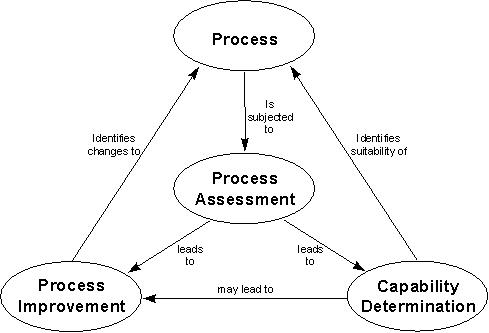
\includegraphics[scale=.6]{img/Spy.png}
		\caption{Modello SPY}
		\label{fig:ModelloSpy}
\end{figure}
\\Lo standard identifica e definisce nove attributi di qualità:
\smallskip
\begin{enumerate}
    \item \textbf{Process performance attribute}: un processo raggiunge i suoi obiettivi, trasformando input identificabili in output identificabili;
    \item \textbf{Performance management attribute}: l'attuazione di un processo è pianificata e controllata al fine di produrre risultati che rispondano agli obiettivi attesi;
    \item \textbf{Work product management attribute}: capacità del processo di elaborare un prodotto documentato, controllato e verificato;
    \item \textbf{Process definition attribute}: l'esecuzione del processo si basa su standard di processo per raggiungere i propri obiettivi;
    \item \textbf{Process resource attribute}: capacità del processo di attingere a risorse tecniche e umane appropriate per essere attuato efficacemente;
    \item \textbf{Process measurement attribute}: i risultati raggiunti e le misure rilevate durante l'attuazione di un processo sono stati usati per assicurarsi che l'attuazione di tale processo supporti efficacemente il raggiungimento di specifici obiettivi;
    \item \textbf{Process control attribute}: il processo viene controllato attraverso la raccolta, analisi ed utilizzo delle misure di prodotto e di processo, al fine di correggere, se necessario, le sue modalità di attuazione;
    \item \textbf{Process change attribute}: i cambiamenti strutturali, di gestione e di esecuzione vengono gestiti in modo controllato;
    \item \textbf{Continuous improvement attribute}: le modifiche al processo sono identificate e implementate per garantire il miglioramento continuo nella realizzazione degli obiettivi di business dell'organizzazione.
\end{enumerate}
\smallskip
La norma definisce poi quattro livelli di possesso di ciascun attributo:
\smallskip
\begin{itemize}
	\item \textbf{N} - Non posseduto (0\%-15\% di possesso): non c'è evidenza oppure ce n'è poca del possesso di un attributo;
	\item \textbf{P} - Parzialmente posseduto (16\%-50\% di possesso): vi è evidenza di approccio sistematico al raggiungimento del possesso di un attributo, ma alcuni aspetti del possesso possono essere non prevedibili;
    \item \textbf{L} - Largamente posseduto (51\%-85\% di possesso): vi è evidenza di approccio sistematico al raggiungimento di un significativo livello di possesso di un attributo, ma l'attuazione del processo può variare nelle diverse unità operative della organizzazione;
	\item \textbf{F} - (Fully) Pienamente posseduto (86\%-100\% di possesso): vi è evidenza di un approccio completo e sistematico e di un pieno raggiungimento del possesso dell'attributo, non esistono significative differenze nel modo di attuare il processo tra le diverse unità operative.
\end{itemize}
\smallskip
Vi sono infine cinque livelli di maturità di processi:
\smallskip
\begin{itemize}
	\item \textbf{Livello 0 - Processo incompleto}: il processo non è implementato o non raggiunge gli obiettivi. Non vi è evidenza di approcci sistematici agli
	attributi definiti;
	\item \textbf{Livello 1 - Processo semplicemente attuato}: il processo viene messo in atto e raggiunge i suoi obiettivi. Non vi è evidenza di un approccio sistematico ad alcuno degli attributi definiti. Il raggiungimento di questo livello è dimostrato attraverso il possesso degli attributi di ``process performance'';
	\item \textbf{Livello 2 - Processo gestito}: il processo è attuato, ma anche pianificato, tracciato, verificato ed aggiustato se necessario, sulla base di obiettivi ben definiti. Il raggiungimento di questo livello è dimostrato attraverso il possesso degli attributi di ``Performance management'' e ``Work product management'';
	\item \textbf{Livello 3 - Processo definito}: il processo è attuato, pianificato e controllato sulla base di procedure ben definite, basate sui principi del software engineering. Il raggiungimento di questo livello è dimostrato attraverso il possesso degli attributi di ``Process definition'' e ``Process resource'';
	\item \textbf{Livello 4 - Processo predicibile}: il processo è stabilizzato ed è attuato all'interno di definiti limiti riguardo i risultati attesi, le performance, le	risorse impiegate ecc. Il raggiungimento di questo livello è dimostrato attraverso il possesso degli attributi di ``Process measurement'' e ``Process control'';
	\item \textbf{Livello 5 - Processo ottimizzante}: il processo è predicibile ed in grado di adattarsi per raggiungere obiettivi specifici e rilevanti per l'organizzazione. Il raggiungimento di questo livello è dimostrato attraverso il possesso degli attributi di ``Process change'' e ``Continuous integration''.
\end{itemize}
Adottando lo standard ISO/IEC$_G$ 15504 gli sviluppatori software del gruppo 	\gruppo\ possono e intendono ottimizzare l'uso delle risorse e contenere così i costi con una migliore stima dei rischi e la possibilità di confrontarsi con delle best practice$_G$.

\subsection{Qualità del Prodotto}
Per quanto concerne la qualità del prodotto si è scelto di seguire alcune linee
guida dettate dallo standard ISO/IEC$_G$ 9126, che definisce la qualità del
prodotto software come l'insieme delle caratteristiche che incidono sulla capacità del prodotto di soddisfare requisiti espliciti o impliciti. Tale standard individua sei caratteristiche indicatrici di qualità del prodotto software, ciascuna delle quali suddivisa in sotto-caratteristiche.
\subsubsection{Funzionalità}
Il prodotto software realizzato deve offrire apposite funzionalità
che siano in grado di soddisfare requisiti funzionali espliciti o impliciti. Le sue sotto-categorie sono:
\begin{itemize}
	\item \textbf{Appropiatezza}: capacità di offrire un insieme di funzioni appropriate per i compiti e gli obbiettivi prefissati all'utente;
	\item \textbf{Accuratezza}: capacità del software di fornire i risultati concordati o i precisi effetti richiesti;
	\item \textbf{Interoperabilità}: capacità di interagire ed operare con altri sistemi;
	\item \textbf{Conformità}: capacità di aderire a standard, convenzioni e regolamentazioni rilevanti al settore operativo in cui viene applicato;
    \item \textbf{Sicurezza}: capacità di proteggere informazioni e dati impedendo gli accessi e le modifiche non autorizzati, mentre garantendo queste operazioni a utenti o sistemi autorizzati.
\end{itemize}
Per misurare il raggiungimento di questo obiettivo si verificherà
la quantità di requisiti soddisfatti che avranno un riscontro in elementi funzionanti nell'applicazione prodotta. La soglia di sufficienza è il soddisfacimento di tutti i requisiti obbligatori previsti dal capitolato d'appalto.
\subsubsection{Affidabilità}
L'affidabilità misura la capacità di un prodotto software di mantenere un determinato livello di prestazioni se usato in determinate condizioni e per un certo periodo.
\begin{itemize}
	\item \textbf{Maturità}: capacità di evitare che si verifichino fallimenti o  malfunzionamenti a causa di errori nel software;
	\item \textbf{Tolleranza agli errori}: capacità di mantenere determinati livelli di prestazioni nonostante l'insorgere di errori, malfunzionamenti o un uso scorretto del prodotto;
	\item \textbf{Recuperabilità}: capacità di ripristinare il livello appropriato di performance e di recuperare le informazioni o dati rilevanti in seguito all'insorgere di un'anomalia;
	\item \textbf{Aderenza}: capacità di aderire a standard, convenzioni e regolamentazioni inerenti l'affidabilità.
\end{itemize}
Per misurare il raggiungimento di questo obiettivo si calcolerà il numero di esecuzioni totale  confrontandolo con quelle andate a buon fine e che hanno mantenuto un livello di prestazioni tali da poter permettere l'utilizzo previsto del prodotto.
\subsubsection{Efficienza}
L'efficienza si misura mettendo in relazione la capacità di fornire prestazioni adeguate con la quantità di risorse impiegate.
\begin{itemize}
	\item \textbf{Comportamento rispetto al tempo}: capacità di fornire tempi di risposta e di elaborazione adeguati per le funzioni richieste, sotto condizioni determinate;
	\item \textbf{Utilizzo delle risorse}: capacità di utilizzare in maniera adeguata la giusta quantità e tipologia di risorse.
\end{itemize}
Il raggiungimento di questo obiettivo sarà misurato dal tempo necessario per ottenere una risposta dal servizio (risposta dell'applicazione più il tempo necessario alla connessione) in condizioni normali e in condizioni di sovraccarico.
\subsubsection{Usabilità}
L'usabilità di un prodotto software si determina in base alla sua capacità di essere capito, appreso e usato dall'utente.
\begin{itemize}
	\item \textbf{Comprensibilità}: costituisce la facilità di comprensione dei concetti del prodotto, permettendo all'utente quindi di comprendere se il programma è appropriato e come può essere utilizzato per compiti specifici compiti;
	\item \textbf{Apprendibilità}: capacità di diminuire l'impegno richiesto agli utenti per imparare ad utilizzare l'applicazione;
	\item \textbf{Operabilità}: capacità di porre gli utenti in condizioni tali da utilizzare il prodotto e controllarne l'uso;
	\item \textbf{Attrattivà}: capacità di essere piacevole e di creare interesse nell'utente;
	\item \textbf{Conformità}: capacità di adesione a standard o convenzioni	relativi all'usabilità.
\end{itemize}
Il raggiungimento di questo obiettivo sarà misurato in base alla capacità dell'applicativo di adattarsi ai vari tipi di ambienti in cui esso verrà eseguito (ambienti desktop o dispositivi mobile). L'usabilità sarà poi ritenuta raggiunta fornendo un'interfaccia il più possibile chiara, semplice ed intuitiva per l'utente.
\subsubsection{Manutenibilità}
La manutenibilità rappresenta la capacità del software di subire modifiche di natura correttiva, miglioramenti o adattamenti, con un impegno contenuto.
\begin{itemize}
	\item \textbf{Analizzabilità}: capacità di facilitare l'analisi del codice e limitare l'impegno richiesto per localizzare un eventuale errore;
	\item \textbf{Modificabilità}: capacità del prodotto di permettere l'implementazione di una specificata modifica;
	\item \textbf{Stabilità}: capacità di evitare effetti inaspettati a seguito delle modifiche apportate;
	\item \textbf{Testabilità}: capacità di essere facilmente testato per validare le modifiche apportate.
\end{itemize}
La misurazione del raggiungimento di questo obiettivo saranno legate al rispetto
delle misure metriche descritte nel capitolo 2.4.3.
\subsubsection{Portabilità}
La portabilità è la capacità di un software d'essere trasferito da un ambiente di
lavoro ad un altro.
\begin{itemize}
	\item \textbf{Adattabilità}: capacità di essere adattato per differenti ambienti operativi eliminando o limitando la necessità di applicare modifiche;
	\item \textbf{Installabilità}: capacità di richiedere il minor impegno possibile per essere installato in uno specifico ambiente;
	\item \textbf{Coesistenza}: capacità di coesistere condividendo risorse con altri software nel medesimo ambiente;
	\item \textbf{Sostituibilità}: capacità di essere utilizzato al posto di un altro software per svolgere gli stessi compiti nello stesso ambiente.
\end{itemize}
L'obiettivo dovrà essere raggiunto ottenendo la compatibilità con i principali browser$_G$ (Google Chrome, FireFox e Internet Explorer) e validando il codice secondo gli standard del W3C$_G$.

\newpage
\section{Gestione amministrativa della revisione}
\subsection{Comunicazione e risoluzione di anomalie}
Un'anomalia corrisponde a:
\begin{itemize}
	\item Violazione delle norme tipografiche da parte di un documento
	\item Incongruenza del prodotto con funzionalità indicate nell'analisi dei requisiti
\end{itemize}
Nel caso in cui un Verificatore o un membro del gruppo individui un anomalia dovrà segnalarlo aprendo un ticket nella forma descritta nella sezione 5.2 delle Norme di Progetto. Un verificatore ha il compito di controllare le pull request quindi nel caso trovasse un anomalia deve bloccare la pull specificando il motivo al richiedente come descritto nella sezione 5.4 delle Norme di Progetto.
\subsection{Trattamento delle discrepanze}
Una discrepanza è un discostamento dai requisiti attesi del capitolato o una violazione delle Norme di Progetto.
Il trattamento delle discrepanze avviene come la gestione delle anomalie. Quando un membro del gruppo o il Verificatore ne individuasse una segnalerà il problema aprendo un ticket oppure un Verificatore può bloccare la pull specificando il motivo al richiedente come per il trattamento delle anomalie.
\subsection{Procedure di controllo di qualità di processo}
Le Procedure di controllo di qualità di processo si basano sul ciclo di Deming o PDCA. Questo garantisce un miglioramento continuo di tutti i processi e delle attività di verifica.
La qualità dei processi viene monitorata anche grazie alla qualità di prodotto perchè un prodotto di bassa qualità può indicare che uno o più processi vanno migliorati.

\newpage
\newcommand{\teststatus}{Pianificato}

\section {Pianificazione dei test}

Si descrivono di seguito tutti i test di validazione, sistema ed integrazione previsti, prevedendo un aggiornamento futuro per i test di unità. Per le tempistiche di esecuzione dei test si faccia riferimento al \textit{Piano di Progetto} v2.0. Nelle tabelle sottostanti lo stato dei test "Pianificato" è da intendersi come non applicato in quanto tali test saranno applicati successivamente, come descritto nel \textit{Piano di Progetto}.

\subsection {Test di sistema}

In questa sezione vengono descritti i test di sistema che permettono di verificare il comportamento dinamico del sistema completo rispetto ai requisiti descritti nell'\textit{Analisi dei Requisiti v2.0}.
I test di sistema riportati sono quelli relativi ai requisiti software individuati e pertanto meritevoli di un test.

\subsubsection{Descrizione dei test di sistema}

\begin{longtable}{|l|p{2.5cm}|p{5cm}|p{3.5cm}|}
\hline
\textbf{Requisito} & \textbf{Stato} & \textbf{Descrizione} & \textbf{Test} \\
\hline
FOb1 & \teststatus & Si verifica che il sistema permetta  la creazione di una presentazione e che questa venga effettivamente creata e salvata sul database & TS1\\
\hline
FOb3 & \teststatus & Si testa l'esecuzione di una presentazione, verificando che il percorso seguito sia quello scelto dall'utente ed il corretto avanzamento delle slides& TS3\\
\hline
FOb3.5 & \teststatus & Si verifica il funzionamento dei checkpoint$_G$, la possibilità per l'utente di impostare un checkpoint$_G$ e il corretto funzionamento dei percorsi di approfondimento & TS3.5  \\
\hline
FOb4 & \teststatus  & Si verifica che le modifiche apportate dall'utente ad una presentazione, quali ad esempio inserimento di oggetti grafici, testi o nuovi frame$_G$ vengano correttamente applicate e salvate dal sistema & TS4 \\
\hline
FOb5 & \teststatus  & Viene verificato che il salvataggio della presentazione avvenga con successo e nel formato atteso & TS5 \\
\hline
FOb6 & \teststatus & Si verifica che l'azione di eliminazione da parte di un'utente di una presentazione cancelli effettivamente tutti i dati relativi a quella presentazione dal sistema & TS6 \\
\hline
FOb6.1 & \teststatus  & Si testa l'annullamento del comando di eliminazione e si verifica che non vi sia alcuna modifica alla presentazione fintanto che l'azione non viene confermata al sistema dall'utente. & TS6.1 \\
\hline
FOb7 & \teststatus & Si verifica che il sistema permetta la pubblicazione di una presentazione e che questa vada a buon fine & TS7 \\
\hline
FOb8 & \teststatus  & Il sistema deve poter generare un link per una presentazione live & TS8 \\
\hline
FOp9 & \teststatus  & l'utente deve poter rendere privata una presentazione pubblica & TS9 \\
\hline
FOb11.1 & \teststatus  & Viene verificato che il sistema permetta di esportare la presentazione in formato poster controllando che il file di output corrisponda alla presentazione esportata &  TS11.1 \\
\hline
FOb11.2 & \teststatus & Si verifica che il formato con cui viene esportata la presentazione sia portabile & TS11.2 \\
\hline
FOb13 & \teststatus  & Si verifica che il sistema permetta all'utente di registrarsi simulando i passi della procedura di registrazione e successivamente verificando il salvataggio dei dati inseriti dall'utente & TS13
\\
\hline
FOb14 & \teststatus  & Si verifica che il sistema permetta all'utente di autenticarsi & TS14 \\
\hline
FOb15 & \teststatus  & Viene verificato il corretto funzionamento di tutti i messaggi di errore da parte del sistema, l'utente deve sapere quando ha commesso un errore & TS15\\
\hline
FOb16 & \teststatus  & Viene verificata e provata la procedura di cambio password, assicurandosi che il sistema salvi correttamente le modifiche dell'utente& TS16\\
\hline
VOb17 & \teststatus  & Viene testato l'avvio del sistema su browser$_G$ Chrome da versione 40+& TS17\\
\hline
\caption{Tabella di tracciamento test di sistema / requisiti}
	
\end{longtable}
\newpage
\subsection {Test di integrazione}

In questa sezione vengono descritti i test di integrazione per i vari componenti descritti nella progettazione ad alto livello, che permettono di verificare la corretta integrazione ed il corretto flusso dei dati all'interno del sistema. Si è scelta una strategia di integrazione incrementale, il cui principale vantaggio è quello di poter sviluppare e verificare le componenti in parallelo.
Con l'approccio incrementale, infatti, i difetti rilevati da un test sono da attribuirsi, con maggior probabilità, all'ultima componente aggiunta ed essendo ogni passo di integrazione reversibile è possibile retrocedere ed effettuare un rollback ad uno stato noto e sicuro.
Per i test di integrazione è stato utilizzato il metodo bottom-up, questa scelta risulta automatica avendola già adottata nella progettazione delle componenti con l'obiettivo quello di ridurre le dipendenze funzionali di ogni singola componente.
Il diagramma seguente non rispetta il formalismo UMLG 2.x ed è utilizzato per semplificare l'illustrazione della strategia di integrazione. Si possono notare, lungo l'albero, dei macro componenti che possono integrare al loro interno due o più componenti di maggior dettaglio.

\begin{figure}[h!]
	\centering
	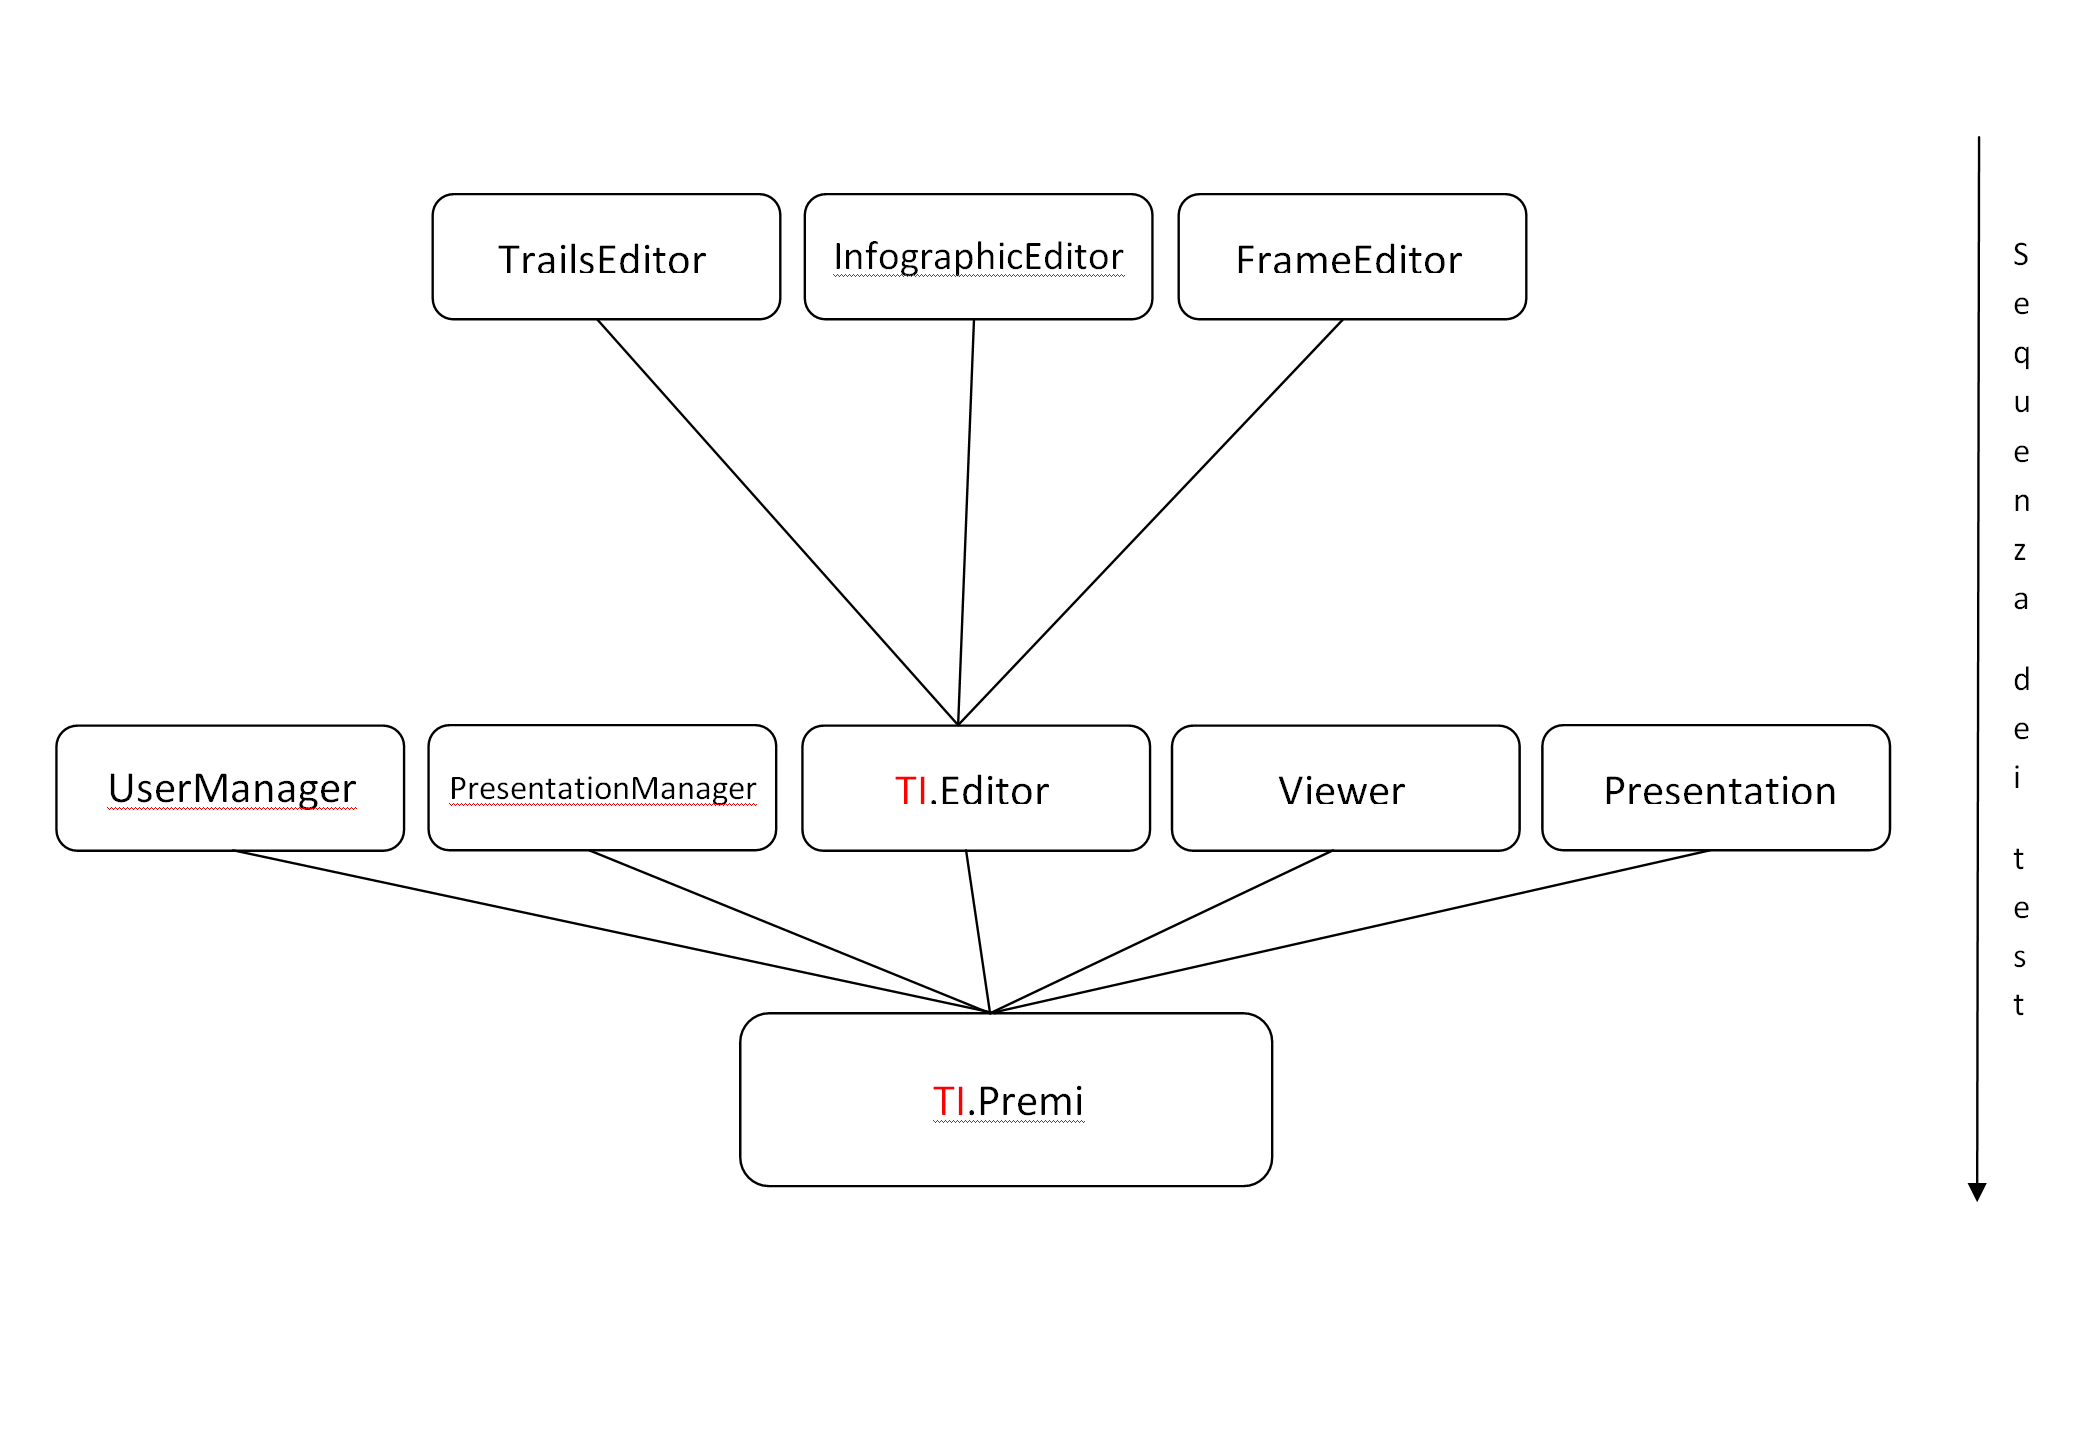
\includegraphics[scale=.45]{img/integrationTests.png}
	\caption{Diagramma informale della strategia di integrazione}
	\label{fig:Diagramma informale della strategia di integrazione}
\end{figure}
\newpage
\subsubsection{Descrizione dei test di integrazione}

\begin{longtable}{|p{4.5cm}|p{7cm}|p{2.5cm}|}
	\hline
	\textbf{Test} & \textbf{Descrizione} & \textbf{Stato} \\
	\hline
	TI.Premi & Test di integrazione finale per le componenti del modulo Premi & \teststatus \\
	\hline
	TI.UserManager & \textbf{Gestione dell'Utente}: Verifica il corretto funzionamento delle operazioni di registrazione, autenticazione e cambio password & \teststatus \\
	\hline
	TI.PresentationManager & \textbf{Gestione della presentazione}: Verifica il corretto funzionamento del sistema di gestione della presentazione, testa la correttezza delle operazioni di creazione, modifica eliminazione, pubblicazione, esportazione e portabilità di una presentazione& \teststatus \\
	\hline
	TI.Editor & Test di integrazione finale per le componenti del modulo Premi::Editor & \teststatus \\
	\hline
	TI.TrailsEditor & \textbf{Edit dei percorsi}: Verifica il corretto funzionamento dei percorsi, e le procedure di creazione, modifica, clonazione ed eliminazione di un persorso & \teststatus \\
	\hline
	TI.InfographicEditor & \textbf{Edit dell'Infografica}: Verifica il corretto funzionamento delle infografiche, nello specifico l'aggiunta di frame$_G$, immagini, testi e shape$_G$ all'infografica e la modifica dello stile& \teststatus \\
	\hline
	TI.FrameEditor & \textbf{Edit dei Frame}: Verifica il corretto funzionamento dei frame$_G$, nello specifico l'aggiunta di immagini, testi e shape$_G$ al frame$_G$ e la modifica dello stile & \teststatus \\
	\hline
	TI.Viewer & \textbf{Visualizzazione della presentazione}: Verifica la corretta riproduzione della presentazione& \teststatus \\
	\hline
	\caption{Tabella test di integrazione}
\end{longtable}

\subsubsection{Tracciamento componenti – test di integrazione}

Nella tabella seguente è riportato il tracciamento delle singole componenti del sistema con il relativo test di integrazione. Si noti che l'integrazione di Views e Controllers sono garantite dall'architettura del sistema.

\begin{longtable}{|l|l|}
	\hline
	\textbf{Componente} & \textbf{Test} \\
	\hline
	Premi & TI.Premi \\
	\hline
	Premi::UserManager & TI.UserManager \\
	\hline
	Premi::UserManager::Views & Architettura del Sistema \\
	\hline
	Premi::UserManager::Controllers & Architettura del Sistema \\
	\hline
	Premi::PresentationManager & TI.PresentationManager \\
	\hline
	Premi::PresentationManager::Views & Architettura del Sistema \\
	\hline
	Premi::PresentationManager::Controllers & Architettura del Sistema \\
	\hline
    Premi::Editor & TI.Editor \\
    \hline
	Premi::Editor::Views & Architettura del Sistema \\
	\hline
	Premi::Editor::Controllers & Architettura del Sistema \\
	\hline
	Premi::Editor::TrailsEditor & TI.TrailsEditor \\
	\hline
	Premi::Editor::TrailsEditor::Views & Architettura del Sistema \\
    \hline
    Premi::Editor::TrailsEditor::Controllers & Architettura del Sistema \\
	\hline
	Premi::Editor::InfographicEditor & TI.InfographicEditor\\
    \hline
    Premi::Editor::InfographicEditor::Views & Architettura del Sistema \\
    \hline
    Premi::Editor::InfographicEditor::Controllers & Architettura del Sistema \\
   	\hline
   	Premi::Editor::FrameEditor & TI.FrameEditor\\
   	\hline
   	Premi::Editor::FrameEditor::Views & Architettura del Sistema \\
   	\hline
   	Premi::Editor::FrameEditor::Controllers & Architettura del Sistema \\
   	\hline
   	Premi::Viewer & TI.Viewer\\
   	\hline
   	Premi::Viewer::Views & Architettura del Sistema \\
   	\hline
   	Premi::Viewer::Controllers & Architettura del Sistema \\
    \hline
	\caption{Tabella tracciamento componente - test di integrazione}
\end{longtable}

\subsection {Test di validazione}

In questa sezione vengono descritti i test di validazione che servono per accertarsi che il prodotto realizzato sia conforme alle attese. Per ogni test vengono descritti i vari passi che un utente deve eseguire per testare i requisiti ad esso associati.

\subsubsection {Test TV1} %registrazione
L'utente vuole verificare che ci si possa registrare al sistema Premi.\\
All'utente è richiesto di:
\begin{itemize}
	\item Aprire il sistema
	\item Navigare nell'area di registrazione
	\item Inserire un indirizzo email. \\
	         All'utente è chiesto di: 
	         \begin{itemize}
	         	\item Verificare che l'inserimento di un indirizzo email non valido generi un avviso da parte del sistema
	         	\item Inserire un indirizzo email valido
	         \end{itemize}
	\item Inserire una password
	\item Reinserire la password per conferma
	\item Verificare che il completamento della registrazione al sistema vada a buon fine
\end{itemize}

\subsubsection {Test TV2} %autenticazione
L'utente vuole verificare il corretto funzionamento dell'autenticazione al sistema Premi\\
All'utente è richiesto di:
\begin{itemize}
	\item Eseguire la registrazione al sistema Premi eseguendo \textbf{TV1}.
	\item Accedere alla sezione di Login del sistema Premi
	\item Inserire un indirizzo email \\
		All'utente è chiesto di: 
		\begin{itemize}
			\item Verificare che l'inserimento di un indirizzo email non valido generi un avviso da parte del sistema
			\item Provare l'inserimento di un indirizzo email diverso da quello fornito in fase di registrazione
		\end{itemize}
	\item Inserire una password\\
	All'utente è chiesto di: 
			\begin{itemize}
				\item Provare l'inserimento di una password diversa da quella fornita in fase di registrazione
				\item Testare la procedura guidata di cambio password (\textbf{TV2.1})
			\end{itemize}
	\item Verificare che in caso di indirizzo mail o password diversi da quelli forniti in fase di registrazione generi un messaggio di errore non facendo terminare a buon fine l'autenticazione.
	\item Verificare che l'autenticazione vada a buon fine e il sistema renda esplicito il successo di questa azione.
\end{itemize}
	 
\subsubsection {Test TV3} % creazione e eliminazione di una presentazione nuova

L'utente vuole testare la creazione di una nuova presentazione e successivamente la sua eliminazione\\
All'utente è richiesto di:
\begin{itemize}
	\item Autenticarsi al sistema Premi eseguendo \textbf{TV2}
	\item Creare una nuova presentazione 
	\item Scegliere ed inserire un titolo per la nuova presentazione (\textbf{TV.3.1}) 
	\item Scrivere una descrizione di almeno di almeno 15 parole per la presentazione (\textbf{TV.3.2})  
	\item Completare la procedura di creazione confermando i dati inseriti
	\item Constatare l'avvenuta creazione della presentazione
	\item Selezionare la presentazione
	\item Eliminare la presentazione selezionata 
	\item Annullare l'operazione di eliminazione prima che questa avvenga effettivamente (\textbf{TV.3.3})
\end{itemize}

\subsubsection {Test TV4} % esecuzione di una presentazione navigazione

L'utente vuole testare l'esecuzione di una presentazione\\
All'utente è richiesto di:

\begin{itemize}
	\item Autenticarsi al sistema Premi eseguendo \textbf{TV2}
	\item Selezionare una presentazione dall'elenco delle presentazioni (\textbf{TV4.1}) 
	\item Scegliere un percorso per la presentazione tra quelli disponibili (\textbf{TV4.2})
	\item Navigare nella presentazione:\\
	All'Utente è chiesto di:
	\begin{itemize}
		\item Avanzare nel percorso presentativo un passo alla volta (\textbf{TV4.3})
		\item Retrocedere nel percorso presentativo un passo alla volta(\textbf{TV4.4}) 
		\item Seguire un percorso di approfondimento a partire da un checkpoint$_G$ (\textbf{TV4.5})
		\item Tornare ad un checkpoint$_G$ dopo aver completato un percorso di approfondimento (\textbf{TV.4.6})
		\end{itemize}
	\item Interrompere l'esecuzione della presentazione (\textbf{TV4.7})
\end{itemize}

\subsubsection {Test TV5} % modifica e salvataggio 

L'utente vuole testare la modifica di una presentazione e il salvataggio delle modifiche\\
All'utente è richiesto di:

\begin{itemize}
	\item Autenticarsi al sistema Premi eseguendo \textbf{TV2}
	\item Selezionare una presentazione dall'elenco delle presentazioni (\textbf{TV4.1})
	\item Entrare nell'editor
	\item Inserire nuovi oggetti grafici nella presentazione (\textbf{TV5.1})\\
	All'utente è chiesto di:
	\begin{itemize}
		\item Provare l'inserimento di un'area di testo (\textbf{TV5.2})\\
		All'utente è chiesto di:
		\begin{itemize}
			\item Inserire un testo di almeno 10 parole  (\textbf{TV5.2.1})
			\item Scegliere un font per il testo (\textbf{TV5.2.2}) 
			\item Scegliere un colore per il testo tra quelli disponibili (\textbf{TV5.2.3})
			\item Scegliere una dimensione diversa da quella di default per il testo (\textbf{TV5.2.4})
		\end{itemize}
       \item Provare l'inserimento di un frame$_G$  (\textbf{TV5.3}) Fob4.1.2\\
        All'utente è chiesto di:		
        \begin{itemize}
        	\item Scegliere una forma tra quelle disponibili per il frame$_G$  (\textbf{TV5.3.1})
        \end{itemize}
        \item Provare l'inserimento di un'immagine  (\textbf{TV5.4})\\
        All'utente è chiesto di:		
        \begin{itemize}
        	\item Scegliere un file immagine da filesystem (\textbf{TV5.4.1})
        \end{itemize}
        \item Provare l'inserimento di uno shape$_G$  (\textbf{TV5.5})\\
        All'utente è chiesto di:		
        \begin{itemize}
        	\item Scegliere una forma tra quelle disponibili per lo shape$_G$ (\textbf{TV5.5.1})
        \end{itemize}
	\end{itemize}
	\item Selezionare un oggetto grafico tra quelli precedentemente inseriti (\textbf{TV5.6})
	\item Provare a modificare un oggetto grafico selezionato (\textbf{TV5.7})\\
	All'utente è chiesto di:
    \begin{itemize}
		\item Provare a modificare un frame$_G$ (\textbf{TV5.8})\\
			All'utente è chiesto di:
			\begin{itemize}
				\item Ridimensionare il frame$_G$ (\textbf{TV5.8.1})
				\item Riposizionare il frame$_G$ (\textbf{TV5.8.2})
				\item Modificare lo stile del frame$_G$  (\textbf{TV5.8.3})
		    \end{itemize}
		 \item Provare a modificare un'area di testo (\textbf{TV5.9})\\
		 	All'utente è chiesto di:
		 	\begin{itemize}
		 		\item Ridimensionare l'area di testo (\textbf{TV5.9.1})
		 		\item Riposizionare l'area di testo (\textbf{TV5.9.2})
		 		\item Modificare lo stile dell'area di testo (\textbf{TV5.9.3})
		 		\item Modificare il contenuto dell'area di testo (\textbf{TV5.9.4})
		 		\item Cambiare il livello dell'area di testo (\textbf{TV5.9.5})
		 	\end{itemize}
		 \item Provare a modificare uno shape (\textbf{TV5.10})\\
		 All'utente è chiesto di:
		 \begin{itemize}
		 	\item Riposizionare lo shape$_G$ (\textbf{TV5.10.1})
		 	\item Ridimensionare lo shape$_G$ (\textbf{TV5.10.2})
		 	\item Modificare lo stile dello shape$_G$ (\textbf{TV5.10.3})
		 	\item Cambiare il livello dello shape$_G$ (\textbf{TV5.10.4})
		 \end{itemize}
		 \item Provare a modificare un'immagine (\textbf{TV5.11})\\
		 All'utente è chiesto di:
		 \begin{itemize}
		 	\item Riposizionare l'immagine (\textbf{TV5.11.1})
		 	\item Ridimensionare l'immagine (\textbf{TV5.11.2})
		 	\item Cambiare il livello dell'immagine (\textbf{TV5.11.3})
		 \end{itemize}
    \end{itemize}
    \item Eliminare un oggetto grafico selezionato (\textbf{TV5.12})
    \item Creare un nuovo percorso per la presentazione (\textbf{TV5.13})\\
    All'utente è chiesto di:
    \begin{itemize}
    	\item Scegliere un titolo per il percorso creato (\textbf{TV5.14})
    	\item Clonare un percorso esistente (\textbf{TV5.15})
    \end{itemize}
    \item Selezionare un percorso tra quelli disponibili (\textbf{TV5.16})
    \item Modificare il percorso selezionato (\textbf{TV5.17})\\
    All'utente è chiesto di:
    \begin{itemize}
    	\item Cambiare il titolo del percorso (\textbf{TV5.18})
    	\item Aggiungere un passo al percorso (\textbf{TV5.19})
    	\item Modificare l'ordine dei frame$_G$ del percorso(\textbf{TV5.20})
    	\item Impostare un frame$_G$ come checkpoint$_G$ (\textbf{TV5.21})
    	\item Rimuovere la marcatura a checkpoint$_G$ da un frame$_G$ (\textbf{TV5.22})\\
    	 All'utente è chiesto di:
    	     \begin{itemize}
    	     	\item Verificare che si debba confermare l'azione intrapresa (\textbf{TV5.22.1})
    	     	\item Verificare che si possa annullare l'azione intrapresa (\textbf{TV5.22.2})
    	     \end{itemize}
    	\item Selezionare un frame$_G$ del percorso del percorso (\textbf{TV5.23})
    \end{itemize}
    \item Eliminare il percorso selezionato (\textbf{TV5.24})
    \item Modificare il titolo di una presentazione (\textbf{TV5.25})
    \item Modificare la descrizione di una presentazione (\textbf{TV5.26})
\end{itemize}


\subsubsection {Test TV6} % esportazione

L'utente vuole verificare il corretto funzionamento dell'esportazione\\
All'utente è richiesto di:

\begin{itemize}
	\item Autenticarsi al sistema Premi eseguendo \textbf{TV2}
	\item Selezionare una presentazione dall'elenco delle presentazioni  (\textbf{TV4.1})
	\item Esportare la presentazione come poster\\
	All'utente è chiesto di:
 \begin{itemize}
 	\item Scegliere uno  dei formati proposti dal sistema per l'esportazione (\textbf{TV6.1})
 	\end{itemize}
	\item Esportare una presentazione in formato portabile\\
	All'utente è chiesto di:
	 \begin{itemize}
	 	\item Verificare che il formato prodotto dal sistema sia portabile e quindi eseguibile offline (\textbf{TV6.2})
	 \end{itemize}
\end{itemize}


\subsubsection {Test TV7} %pubblicazione

L'utente vuole verificare il corretto funzionamento della pubblicazione di una presentazione\\
All'utente è richiesto di:

\begin{itemize}
	\item Autenticarsi al sistema Premi eseguendo \textbf{TV2}
	\item Selezionare una presentazione dall'elenco delle presentazioni (\textbf{TV4.1})
	\item Pubblicare la presentazione
	\item Verificare che il sistema generi un link alla presentazione e lo renda noto all'utente (\textbf{TV7.1})
\end{itemize}
\newpage
\subsubsection {Tracciamento Test di Validazione - Requisiti}

\begin{longtable}{|p{2.5cm}|p{5cm}|}
\hline
\textbf{Requisito} & \textbf{Test di Validazione} \\
\hline
Fob13 & TV1\\
\hline
Fob14 & TV2\\
\hline
FOb16 & TV2.1\\
\hline
FOb1 & TV3\\
\hline
FOb1.1 & TV3.1\\
\hline
FOb1.2 & TV3.2\\
\hline
FOb6& TV3\\
\hline
FOb6.1 & TV3.3\\
\hline
FOb3 & TV4\\
\hline
FOb2 & TV4.1\\
\hline
FDe3.1 & TV4.2\\
\hline
FOb3.2 & TV4.3\\
\hline
FOb3.3 & TV4.4\\
\hline
FDe3.4 & TV4.5\\
\hline
FOb3.5 & TV4.6\\
\hline
FOb3.6 & TV4.7\\
\hline
FOb4 & TV5\\
\hline
FOb4.1 & TV5.1\\
\hline
FOb4.1.1 & TV5.2\\
\hline
FOb4.1.1.1 & TV5.2.1\\
\hline
FOb4.1.1.2 & TV5.2.2\\
\hline
FOb4.1.1.3 & TV5.2.3\\
\hline
FOb4.1.1.4 & TV5.2.4\\
\hline
FOb4.1.2 & TV5.3\\
\hline
FOb4.1.2.1 & TV5.3.1\\
\hline
FOb4.1.3 & TV5.4\\
\hline
FOb4.1.3.1 & TV5.4.1\\
\hline
FOb4.1.4 & TV5.5\\
\hline
FOb4.1.4.1 & TV5.5.1\\
\hline
FOb4.2 & TV5.6\\
\hline
FOb4.3 & TV5.7\\
\hline
FOb4.3.1 & TV5.8\\ %frame
\hline
FOb4.3.1.1 & TV5.8.1\\
\hline
FOb4.3.1.2 & TV5.8.2\\
\hline
FOb4.3.1.3 & TV5.8.3\\
\hline
FOb4.3.3 & TV5.9\\ %area testo
\hline
FOb4.3.3.1 & TV5.9.1\\
\hline
FOb4.3.3.2 & TV5.9.2\\
\hline
FOb4.3.3.3 & TV5.9.3\\
\hline
FOb4.3.3.4 & TV5.9.4\\
\hline
FOb4.3.3.5 & TV5.9.5\\
\hline
FOb4.3.4 & TV5.10\\ %shape
\hline
FOb4.3.4.1 & TV5.10.1\\
\hline
FOb4.3.4.2 & TV5.10.2\\
\hline
FOb4.3.4.3 & TV5.10.3\\
\hline
FOb4.3.4.4 & TV5.10.4\\
\hline
FOb4.3.2 & TV5.11\\ %immagine
\hline
FOb4.3.2.1 & TV5.11.1\\
\hline
FOb4.3.2.2 & TV5.11.2\\
\hline
FOb4.3.2.3 & TV5.11.3\\
\hline
FOb4.4 & TV5.12\\ %eliminazione
\hline
FDe4.5 & TV5.13\\ %crea percorso
\hline
FDe4.5.1 & TV5.14\\  %titolo pres
\hline
FDe4.5.2 & TV5.15\\ %clona
\hline
FDe4.6 & TV5.16\\ %selez perorso
\hline
FOb4.7 & TV5.17\\ %modifica perorso
\hline
FDe4.7.1 & TV5.18\\ %titolo perorso
\hline
FOb4.7.2 & TV5.19\\ %add passo perorso
\hline
FOb4.7.3 & TV5.20\\ %ordine frame perorso
\hline
FDe4.7.4 & TV5.21\\ %check perorso
\hline
FDe4.7.5 & TV5.22\\ %rm chek frame 
\hline
FDe4.7.5.1 & TV5.22.1\\ %rm chek frame 
\hline
FDe4.7.5.2 & TV5.22.2\\ %rm chek frame 
\hline 
FOb4.7.6 & TV5.23\\ % sel frame
\hline 
FDe4.9 & TV5.24\\ %elimina perc
\hline
FOb4.8 & TV5.25\\ %titolo pres
\hline
FOb4.10 & TV5.26\\%descr pres
\hline
FOb11 & TV6\\
\hline
FOb11.1 & TV6.1\\
\hline
FOb11.2 & TV6.2\\	
\hline
FOb7 & TV7\\
\hline
FOb8 & TV7.1\\
\hline
\end{longtable}









\newpage
\appendix
\section{Resoconto dell' Attività di Verifica}
In questa sezione vengono descritte le procedure adottate durante il processo di
verifica e i risultati ottenuti.
\subsection{Revisione della Documentazione}
Riguardo all'attività di verifica della documentazione, la checklist stilata dai verificatori durante i controlli sui documenti tramite Inspection è la seguente:\\ \\
\textbf{Per i documenti in \LaTeX}:
\begin{itemize}
	\item[-] assenza di doppi spazi;
	\item[-] uso corretto delle lettere maiuscole e minuscole negli elenchi puntati e all'inizio di ogni frase;
	\item[-] assenza di errori ortografici di battitura;
	\item[-] presenza dello spazio dopo il segno di punteggiatura; 
	\item[-] assenza di parti mancanti nei documenti;
	\item[-] mancanza nel glossario della spiegazione di termini segnati $_G$ nei documenti;
	\item[-] evitare di scrivere frasi troppo lunghe;
	\item[-] evitare l'inserimento di spazi nei tag \LaTeX{};
	\item[-] assenza di spazi all'apertura e alla chiusura delle parentesi tonde o quadre;
	\item[-] presenza dello spazio dopo i segni di punteggiatura; 
	\item[-] verifica del funzionamento dei link dei documenti.
\end{itemize}
\textbf{Per i diagrammi UML$_G$}:
\begin{itemize}
	\item[-] il sistema non deve essere un attore;
	\item[-] direzione delle freccie scorretta;
	\item[-] controllo ortografico.
\end{itemize}
\subsection{Tracciamento requisiti}
Il tracciamento dei requisiti viene eseguita tramite il software 404TrackerDB descritto nella sezione 2.4.1. 
Grazie anche allo strumento TexMaker$_G$ descritto nella sezione 2.4.1 si è potuto individuare errori ortografici mentre la parte di controllo grammaticale è avvenuta mediante la rilettura da parte dei verificatori dei documenti. I verificatori nel segnalare gli errori hanno emesso i ticket ai redattori che sono stati poi risolti dagli stessi.
Ciò che si è controllato viene descritto dalla lista seguente:
\begin{itemize}
\item[-] ad ogni use case$_G$ deve corrispondere un requisito;
\item[-] ad ogni requisito deve corrispondere la sua fonte;
\item[-] i requisiti devono coprire l'intero capitolato;
\item[-] Ogni requisito deve avere un codice univoco;
\item[-] i codici dei casi d'uso nei diagrammi devono corrispondere;
\item[-] la numerazione dei casi d'uso non deve contenere salti.
\end{itemize}
I requisiti presenti nel documento AnalisiDeiRequisiti.pdf sono:
\begin{itemize}
\item \textbf{Totali}: 
\item \textbf{Funzionali utente}:
\item \textbf{Funzionali amministratore}:
\item \textbf{di Vincolo}:
\item \textbf{di Qualità}:
\end{itemize}
Gli use case$_G$ individuati sono ???  di cui lato utente ??? e ??? lato  amministratore.
\subsection{Dettaglio delle verifiche tramite analisi}
La verifiche tramite analisi statica avvengono con le modalità walkthrough e inspect spiegate sezione 2.4.2 e permettono di controllare l'andamento e la qualità del lavoro svolto.

\bibliography{../bibliography}
\end{document}
